\documentclass[
  lualatex,
  aspectratio=169,
  14pt
]{beamer}

\usetheme[progressbar=frametitle]{Metropolis}
%\setbeameroption{show notes on second screen=bottom}

\usepackage{xparse}
\usepackage{mathtools,amssymb}
\usepackage{graphicx,xcolor}
\usepackage{pxrubrica}
\usepackage{calc}
\usepackage[absolute,overlay]{textpos}
\usepackage{enumitem}
\usepackage[1.7]{bxpdfver}
\usepackage{pdfcomment}
\usepackage{ulem}
\usepackage{stackengine}
\usepackage{appendixnumberbeamer}

% フォント
\usepackage[lining,tabular,sfdefault]{FiraSans}
\usepackage[mathrm=sym,mathbf=sym]{unicode-math}
\setmathfont{Fira Math}
\usepackage[no-math,deluxe,haranoaji]{luatexja-preset}
\RenewDocumentCommand\kanjifamilydefault{}{\gtdefault}

% 打ち消し線関連
\RenewDocumentCommand\ULthickness{}{.1\zh}
% 二重打ち消し
\NewDocumentCommand\dsout{m}{%
  \stackengine{.2\zh}{#1}{%
    \stackengine{-.3\zh}{\sout{\hphantom{#1}}}{\sout{\hphantom{#1}}}{O}{c}{F}{F}{L}%
  }{O}{c}{F}{F}{L}}

% 下に文字置くやつ
\NewDocumentCommand\replace{mm}{%
  \smash{\stackengine{-1\zh}{\dsout{#1}}{#2}{O}{c}{F}{F}{L}}}

\usepackage{hyperref}

\title{オレオレIP電話網を大きくしたら\\
Tailscaleの\texorpdfstring{\replace{不具合}{ワナ}}{ワナ}を踏み抜いて発狂した話\\
\hfill(再放送版)}
\subject{CS集会\#53}
\author{上羽 未栞(a.k.a. KusaReMKN)}
\institute{%
  \href{https://tkytel.github.io/}{東京広域電話網〈\url{https://tkytel.github.io/}〉}\\
  \url{https://KusaReMKN.com/}\\
  Twitter: \href{https://twitter.com/KusaReMKN}{@KusaReMKN}}
\keywords{Tailscale; 黒電話; VoIP; IP電話; MikoPBX; 東京広域電話網}
\date{2025-06-03}

\begin{document}

\begin{frame}
  \titlepage
  \note{
    発表を始めるよ。
    「オレオレIP電話網を大きくしたらTailscaleのワナを踏み抜いて発狂した話」と題して、
    みかんちゃんが発表するよ。
  }
\end{frame}

\begin{frame}
  \frametitle{今回のおはなし}

  ~\\[-.25\baselineskip]
  \tableofcontents
  \note{
    今回の発表の流れはこんな感じだよ。
    質疑応答を含めて大体20分間くらいで進められたらいいな。
  }
\end{frame}

\section*{みかんちゃんについて}
\note{
  自己紹介するよ。
}

\begin{frame}
  \frametitle{自称・大天才美少女プログラミング初心者}

  \begin{textblock*}{0.5\paperwidth}(0.6cm, 3.5cm)
    
\includegraphics[width=0.3\paperwidth]{./images/mikanchan.png}
  \end{textblock*}
  \begin{columns}
    \begin{column}{0.30\textwidth}
      \\~\\[-.25\baselineskip]
    \end{column}
    \begin{column}{0.69\textwidth}
      \\~\\[-.25\baselineskip]
      「\ruby{上羽}{うわ|ば} \ruby{未栞}{み|かん}」
      あるいは「\ruby[g]{KusaReMKN}{くされみかん}」\\
      \hspace{1.5\zw}\textbf{みかんちゃん}って呼んでね!
      \\~\\[-.5\baselineskip]

      実はプログラマでもエンジニアでもない\\
      \hspace{1.5\zw}古い計算機っぽいものが大好き\\
      \hspace{1.5\zw}最近は電話機などにも目がない
      \\~\\[-.5\baselineskip]

      Twitterで思想を垂れ流すことが得意\\
      \hspace{1.5\zw}\url{https://kusaremkn.com/}も見てね
    \end{column}
  \end{columns}
  \note{
    大天才美少女プログラミング初心者を自称している、上羽未栞だよ。
    みかんちゃんって呼ばれると大変喜ぶよ。

    大天才とかプログラミング初心者とか言っているけれど、
    実はプログラマでもエンジニアでもないよ。
    外の人(学生のすがた)は通信方式について研究していたりするけれど、
    それはまた別のお話だよ。
    それはそれとして古い計算機っぽいものが大好きだよ。
    よくハードオフに出没してジャンク箱を小豆洗いしているよ。
    最近は電話機などにもお熱で、家に電話機が20台以上発生していて困っているよ。

    Twitterとかウェブサイトとかあるよ。
    暇な人は覗いてみてね。
    深淵があるよ。
  }
\end{frame}

\section{東京広域電話網について}
\note{
  みかんちゃんたちがやっているオレオレIP電話網「東京広域電話網」について説明するよ。
}

\begin{frame}
  \frametitle{分散型の異常オレオレIP電話網}

  \textbf{東京広域電話網}
  (\textit{Tokyo Wide Area Telephony Network})\\
  \hspace{1.5\zw}Telephone for Everyone, Connecting Heritages
  \\~\\[-.5\baselineskip]

  2024年10月頃に発足したオレオレIP電話網\\
  \hspace{1.5\zw}VoIPサーバを設置して相互接続・電話網を構築\\
  \hspace{1.5\zw}黒電話やワープロなど異常な端末が数多く生息中
  \\~\\[-.5\baselineskip]

  2月21日のエンジニア作業飲み集会でLT発表\\
  \hspace{1.5\zw}電話局の数: 13 → 34\\
  \hspace{2.5\zw}端末の数: 58 → 234\\
  \hspace{1.5\zw}(2025-06-01 14:14現在)

  \note{
    東京広域電話網は分散型のオレオレIP電話網だよ。
    Telephone for Everyone, Connecting Heritagesをスローガンに、
    故き良き通信を楽しんでいるよ。

    東京広域電話網のプロジェクトは去年の10月に始まって、
    各人が各々の電話サーバを立てて相互に接続することで電話網を形成しているよ。
    黒電話やワープロなどの異常な端末が数多く生息しているよ。

    2月にエンジニア作業飲み集会でLTをしたときに大反響があって、
    それ以来網がだい成長しているよ(だいたい、全ての数字が倍になったよ)。
  }
\end{frame}

\begin{frame}
  \frametitle{現在の東京広域電話網の姿}

  \begin{columns}
    \begin{column}{.28\textwidth}
      \begin{description}[labelwidth=\linewidth]
        \item[交換局数]
          34局
        \item[端末数]
          234以上\\
          (仮想含む)
        \item[うち黒電話]
          29程度?
        \item[その他]
          ピンク電話\\
          ISDNやPHS
      \end{description}
    \end{column}
    \begin{column}{.7\textwidth}
      \centering
      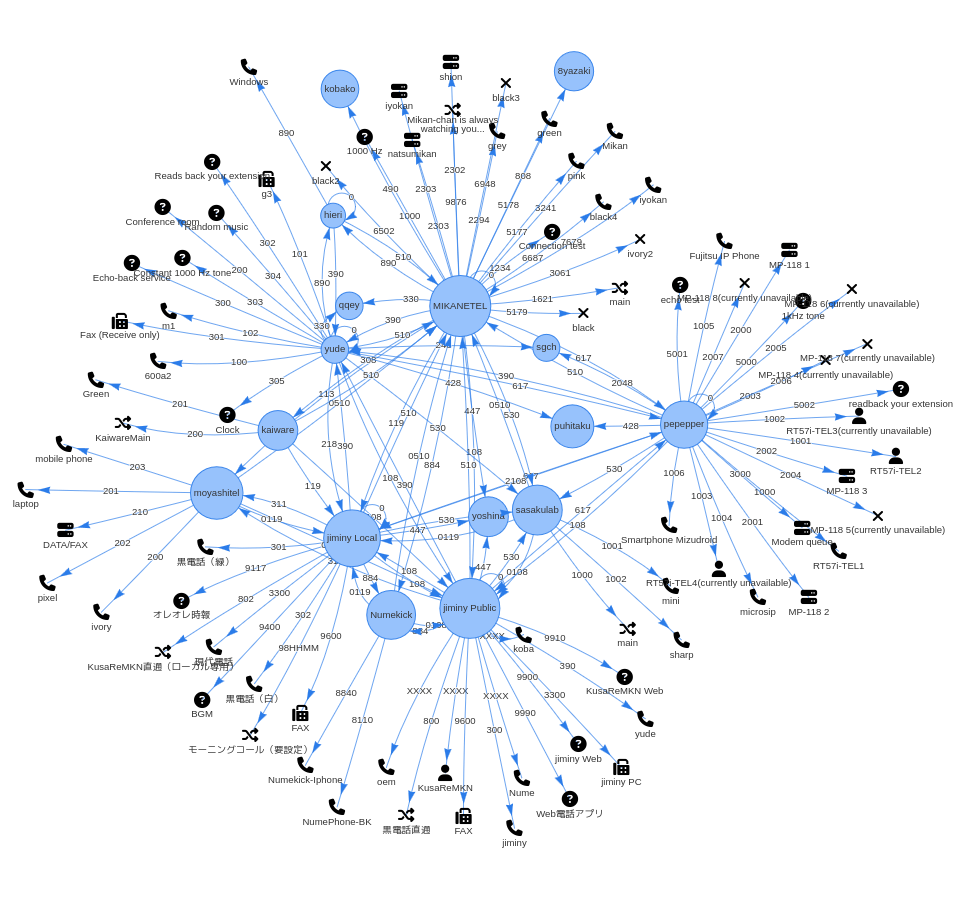
\includegraphics[height=.9\textheight]{./images/mantela.png}
    \end{column}
  \end{columns}

  \note{
    東京広域電話網の現在の姿を図に示すとこんな感じになるよ。
    ネットワークが複雑でちょっと見づらいのは許してね。
  }
\end{frame}


\begin{frame}
  \frametitle{さまざまな東京}

  \centering
  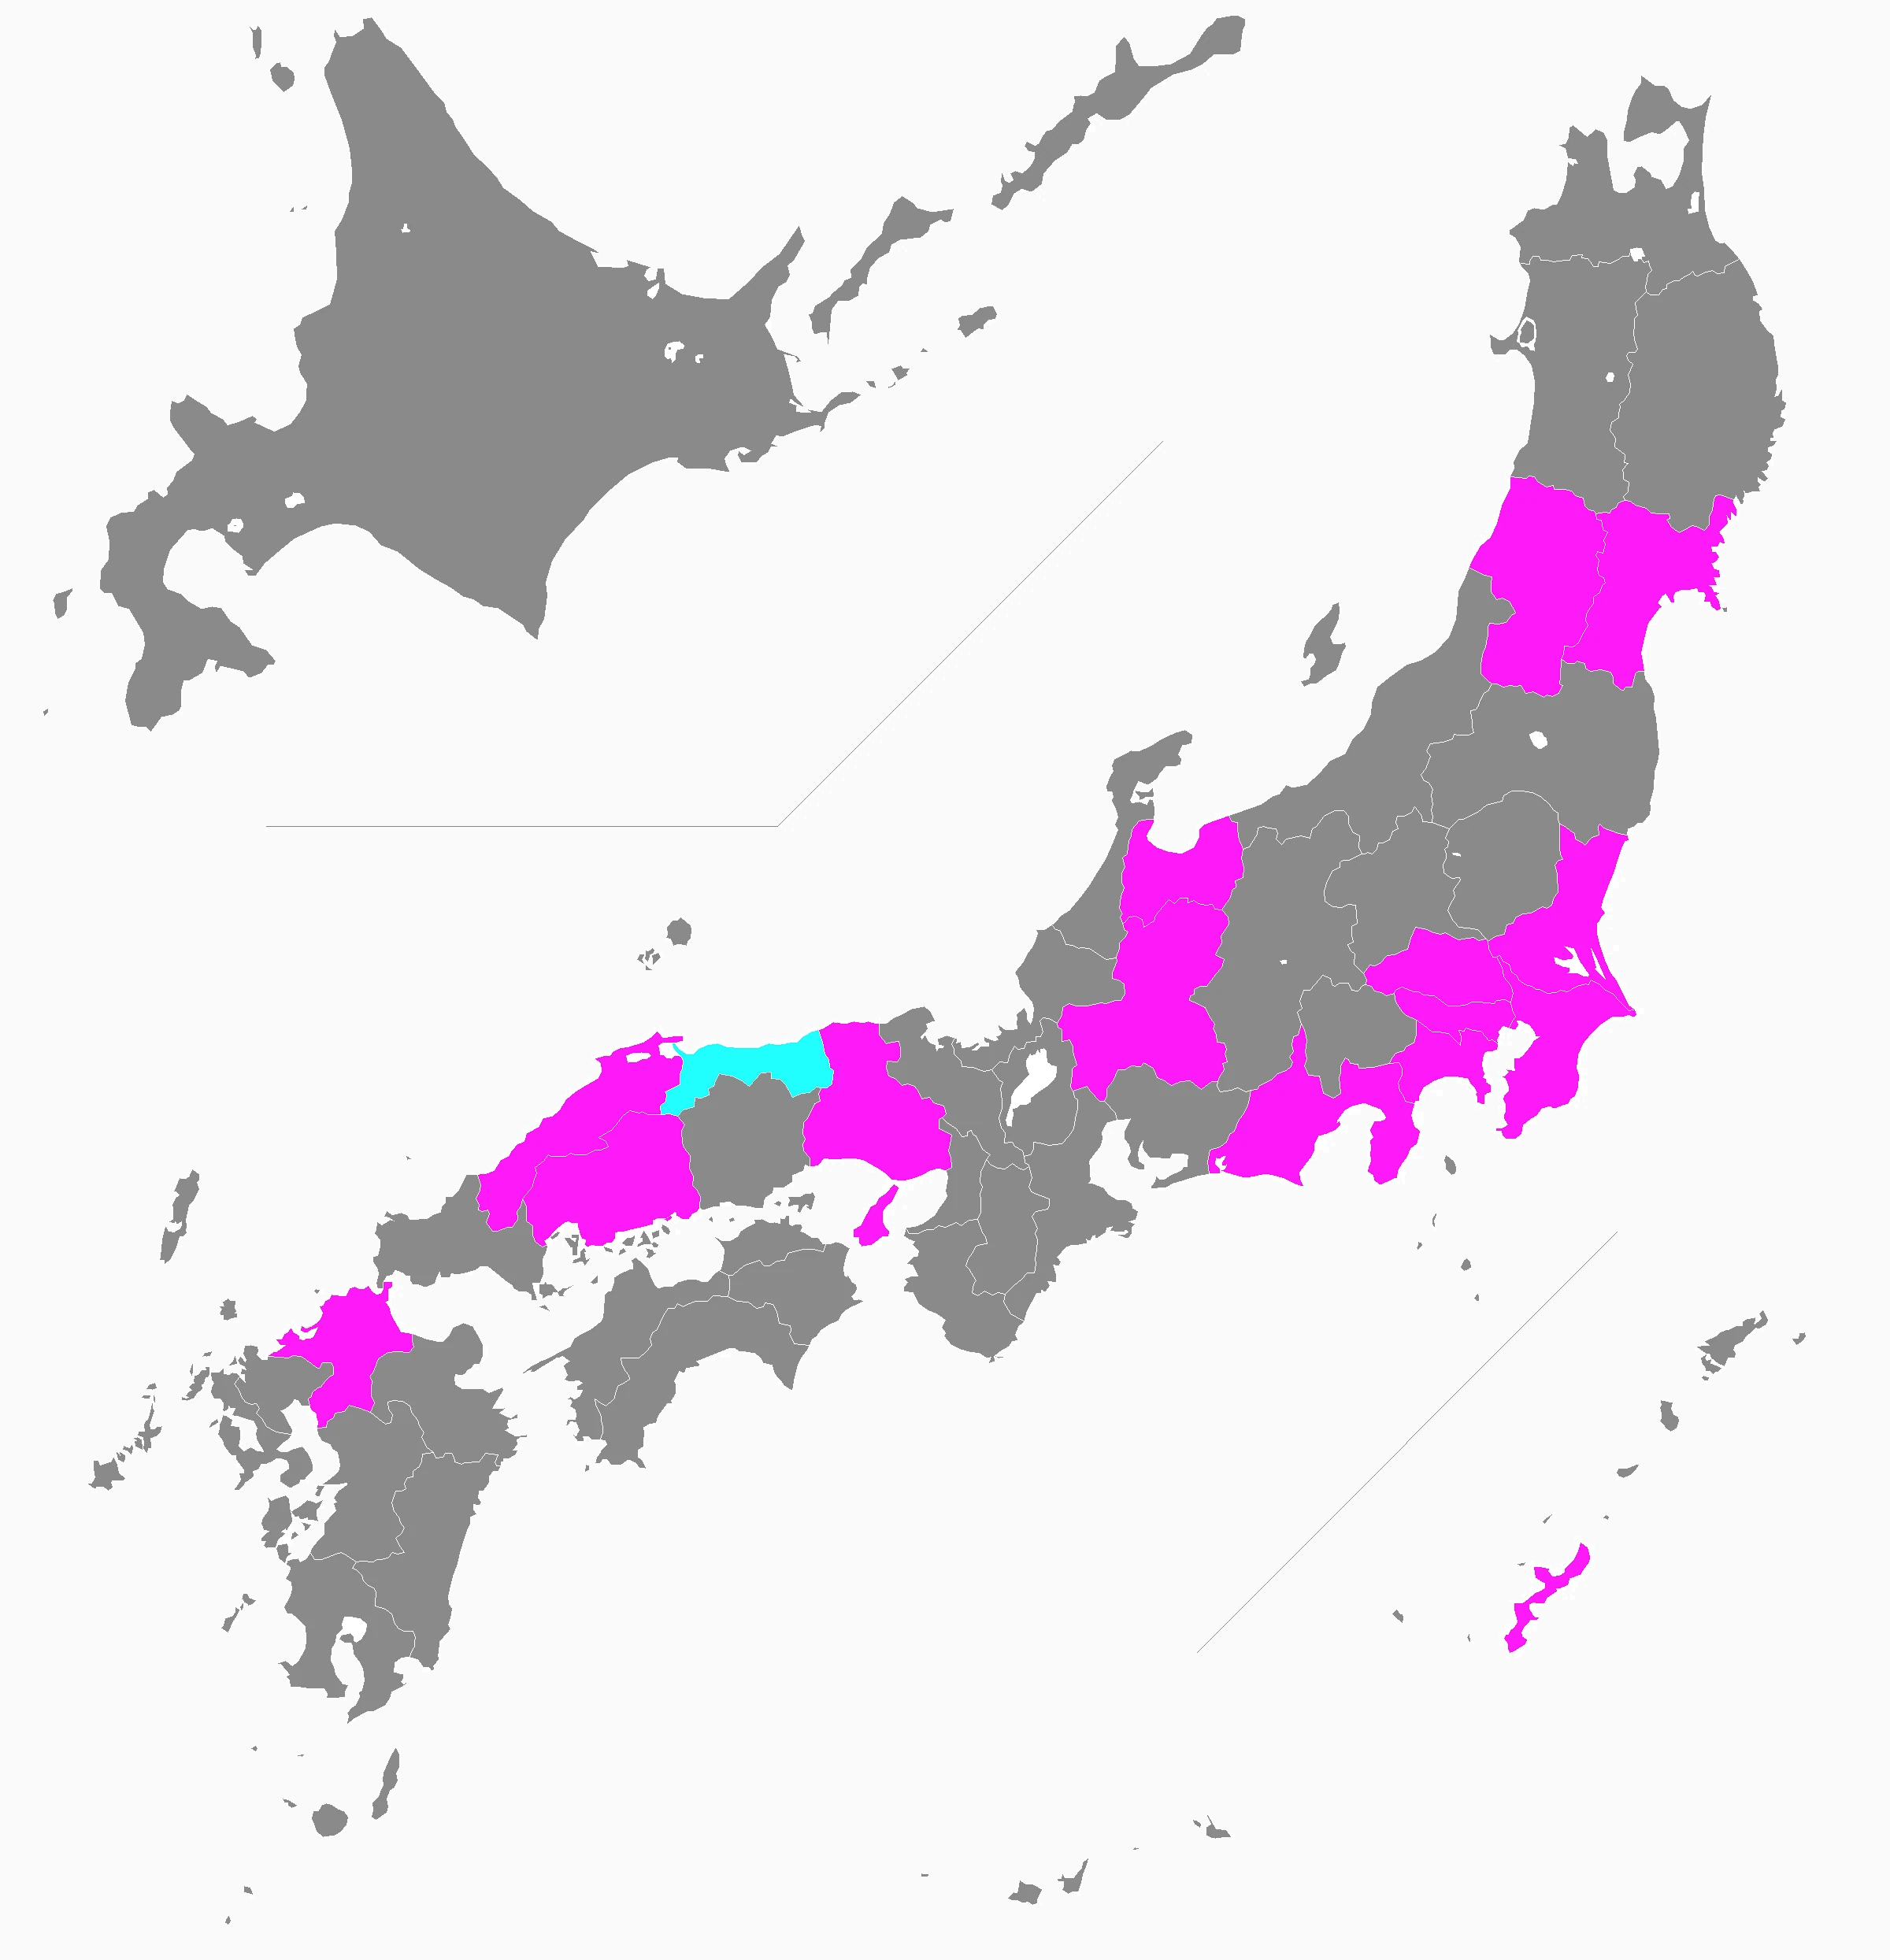
\includegraphics[height=\textheight]{./images/map.png}

  \note{
    東京ってさまざまなところにあります
  }
\end{frame}


\begin{frame}
  \frametitle{東京広域電話網コミュニティ}

  \begin{description}[labelwidth=\linewidth]
    \item[Website]
      {\small
      \url{https://tkytel.github.io/}}
    \item[VRChat Group]
      {\small
      \href{https://vrc.group/TKYTEL.6282}{TKYTEL.6282}}
    \item[Discord]
      {\small
      \url{https://discord.com/invite/QEzAnuSy9S}}
    \item[GitHub Organization]
      {\small
      \url{https://github.com/tkytel}}
    \item[Mailing list]
      {\small
      \url{https://groups.google.com/g/tkytel}}
  \end{description}
  \note{
    東京広域電話網のコミュニティがあるよ。
    気軽に参加してみてね。
    VRChat Groupもできたよ!
  }
\end{frame}

\begin{frame}
  \frametitle{技術的なおはなし}

  \begin{description}[labelwidth=\linewidth]
    \item[いまさらVoIP網]
      {\small
      \url{https://zenn.dev/kusaremkn/articles/abd760f9f2f450}}
    \item[VoIPルータを使って黒電話をIP電話機にする]
      {\small
      \url{https://zenn.dev/kusaremkn/articles/187222dc1d4f1d}}
    \item[ICOM VE-TA10を使うためにパケットを書き換えたりする]
      {\small
      \url{https://zenn.dev/kusaremkn/articles/cb32b500fc1334}}
    \item[AudioCodes MP-118 VoIP GatewayをMikoPBXに収容する]
      {\small
      \url{https://zenn.dev/pepepper/articles/b8ad94b4b6f05f}}
  \end{description}
  \note{
    いまさらVoIP網でGoogleすると引っ掛かるハズなので、
    でんわをしてみたい人は検索してみてね。
    ほかにもいろいろあるよ。
  }
\end{frame}

\section{東京広域電話網の電話局同士の接続}
\note{
  東京広域電話網における電話局同士の接続について簡単に説明するよ。
}

\begin{frame}
  \frametitle{基本の構成}

  \begin{columns}
    \begin{column}{.6\textwidth}
      交換局として\textbf{MikoPBX}を用いる\\
      \hspace{1.5\zw}AsteriskベースのIP PBXシステム
      \\~\\[-.5\baselineskip]

      \textbf{Proxmox}や\textbf{Docker}を利用して\\
      \hspace{1.5\zw}コンテナ環境を構築
      \\~\\[-.5\baselineskip]

      交換局同士の相互接続には\\
      \hspace{1.5\zw}VPNサービス\textbf{Tailscale}を用いる
    \end{column}
    \begin{column}{.39\textwidth}
      
\includegraphics[width=\linewidth]{./images/mikopbx.png}
      \\~\\

      
\includegraphics[width=\linewidth]{./images/docker.png}
      \\~\\

      
\includegraphics[width=\linewidth]{./images/tailscale.png}
    \end{column}
  \end{columns}
  \note{
    東京広域電話網の交換局の多くは、
    MikoPBXというAsteriskベースのIP PBXシステムを利用しているよ。
    MikoPBXを動作させる環境を構築するために
    ProxmoxやDockerなどのコンテナ仮想化技術を利用しているよ。
    また、網内の他の交換局と相互に接続するために、
    メッシュ形のVPNサービスであるTailscaleを利用しているよ。
  }
\end{frame}

\begin{frame}
  \frametitle{システム構成図}

  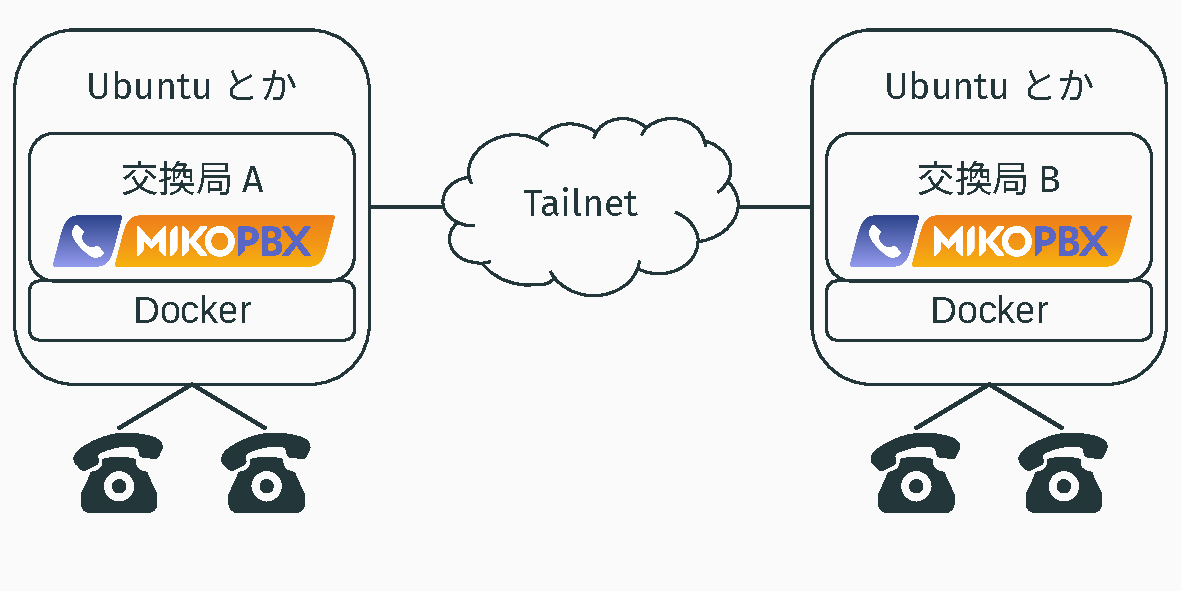
\includegraphics[page=1,width=\linewidth]{./images/pictures.pdf}

  \note{
    システム構成を簡単な図に表すとこのようになるよ。
    Ubuntuなど適当なホスト環境の上にDocker環境を用意し、
    その上でMikoPBXを動作させているよ。
    また、それぞれの局を接続するためにTailnetに接続しておくよ。
  }
\end{frame}

\begin{frame}
  \frametitle{交換局をホップするような通話にも対応}

  \includegraphics[page=2,width=\linewidth]{./images/pictures.pdf}
  \note{
    東京広域電話網では直接相互接続されていないような局同士でも
    通信できる仕組みを用意しているよ。
    これを交換局ホップと呼んでいるよ。
    交換局ホップを利用すると、
    直接相互接続されていないような局間の通信であっても、
    別の局を踏み台にして通信を実現することができるよ。
  }
\end{frame}

\section{網内のセキュリティ強化(素振り)}
\note{
  ここまで東京広域電話網の概要についてお話してきたので、
  ここから本編を始めていくよ。
}

\begin{frame}
  \frametitle{電話網内のセキュリティを向上しよう}

  東京広域電話網も最初は身内向けの小規模電話網だった\\
  \hspace{1.5\zw}網内のユーザは全員信頼されていることが前提
  \\~\\[-.5\baselineskip]

  時代は変わって大規模電話網になってしまった\\
  \hspace{1.5\zw}網内に悪意を持ったユーザが登場するおそれが出てきた\\
  \hspace{1.5\zw}(東京広域電話網はお前らを信じていますよ)
  \\~\\[-.5\baselineskip]

  → 網内のセキュリティを向上するための施策が必要

  \note{ }
\end{frame}

\begin{frame}
  \frametitle{懸念事項: Tailscaleでホストを共有している}

  電話局を相互接続するためにTailscaleを利用\\
  \hspace{1.5\zw}基本的には電話局のホストそれ自体を共有\\
  \hspace{1.5\zw}何もしていないとそのホストの全てが見える
  \\~\\[-.5\baselineskip]

  例えば……\\
  \hspace{1.5\zw}他局のMikoPBXの設定画面(Web UI)にアクセスできる\\
  \hspace{1.5\zw}MikoPBXをホストしているコンテナにSSHできる\\
  \hspace{1.5\zw}電話に関係のないサービスまで露出する
  \\~\\[-.5\baselineskip]

  \hfill ↑ なんかちょっと怖そう(かなり怖そう)

  \note{ }
\end{frame}

\begin{frame}
  \frametitle{Tailscaleを使っているのだからTailscale ACLを使おう}

  Tailscale ACL(Access Control List)とは\\
  \hspace{1.5\zw}Tailnet上でアクセス制御をする手段
  \\~\\[-.5\baselineskip]

  Deny by defaultからアクセス許可するルールを列挙する\\
  \hspace{1.5\zw}初期状態では全アクセスを許可するルールを設定済

  \note{ }
\end{frame}

\begin{frame}
  \frametitle{とりあえず東京広域電話網の二大巨頭で実験}

  yude局及びMikaNeTEL局に設定して試験運用\\
  \hspace{1.5\zw}……が、なんかうまくいかない\\
  \hspace{1.5\zw}挙句の果てにはyude-MikaNeTEL間の通信ができなくなる\\
  \hspace{1.5\zw}→ 交換局ホップに頼っている経路に影響
  \\~\\[-.5\baselineskip]

  全てを元に戻してほぼ初期状態へ\\
  \hspace{1.5\zw}MikoPBXに付属しているFirewallを利用する方針へ変更\\
  \hspace{1.5\zw}コンテナをhostモードで運用しているためこれで良かった

  \note{ }
\end{frame}

\section{不思議な不通問題}
\note{ }

\begin{frame}
  \frametitle{新規局参入 → 不通}

  いつものように東京広域電話網に新規局が参入\\
  \hspace{1.5\zw}接続確認のための自動応答番号を設置しがち\\
  \hspace{1.5\zw}ノウハウがぼんやりとしているのでたびたび事故が起きる
  \\~\\[-.5\baselineskip]

  例によって今回も確認用の番号に掛けるも無音\\
  \hspace{1.5\zw}よくあるトラブルシューティングのノリで対応開始\\
  \hspace{1.5\zw}設定項目を確認するもこれといって問題点は見付からず\\
  \hspace{1.5\zw}どうしようもないので人対人通信で接続を確認することに

  \note{ }
\end{frame}

\begin{frame}
  \frametitle{前例のない不具合: ベルは鳴れど通話はできず}

  相手に電話を掛けると「プルプルプル」の音が鳴る\\
  \hspace{1.5\zw}電話の受け側でもベルが鳴っている
  \\~\\[-.5\baselineskip]

  相手が受話器を上げたらしく「プルプルプル」の音が止む\\
  \hspace{1.5\zw}とりあえず「もしもし」してみる\\
  \hspace{1.5\zw}電話の受け側では「もしもし」が聞こえる\\
  \hspace{1.5\zw}しかし返事は聞こえない(しばらくすると通話が切れる)

  \note{ }
\end{frame}

\begin{frame}
  \frametitle{IP電話のウラ側: 呼制御のSIPと実通信のRTP}

  \begin{columns}
    \begin{column}{.35\textwidth}
      ベルが鳴っている\\
      \hspace{1\zw}→ SIPはOKっぽい
      \\~\\[-.5\baselineskip]

      声が聞こえない\\
      \hspace{1\zw}→ RTPが死んでる
      \\~\\[-.5\baselineskip]

      勝手に通話が切れる\\
      \hspace{1\zw}→ だんまりだから
    \end{column}
    \begin{column}{.65\textwidth}
      \raggedleft
      ~\\[.2\baselineskip]
      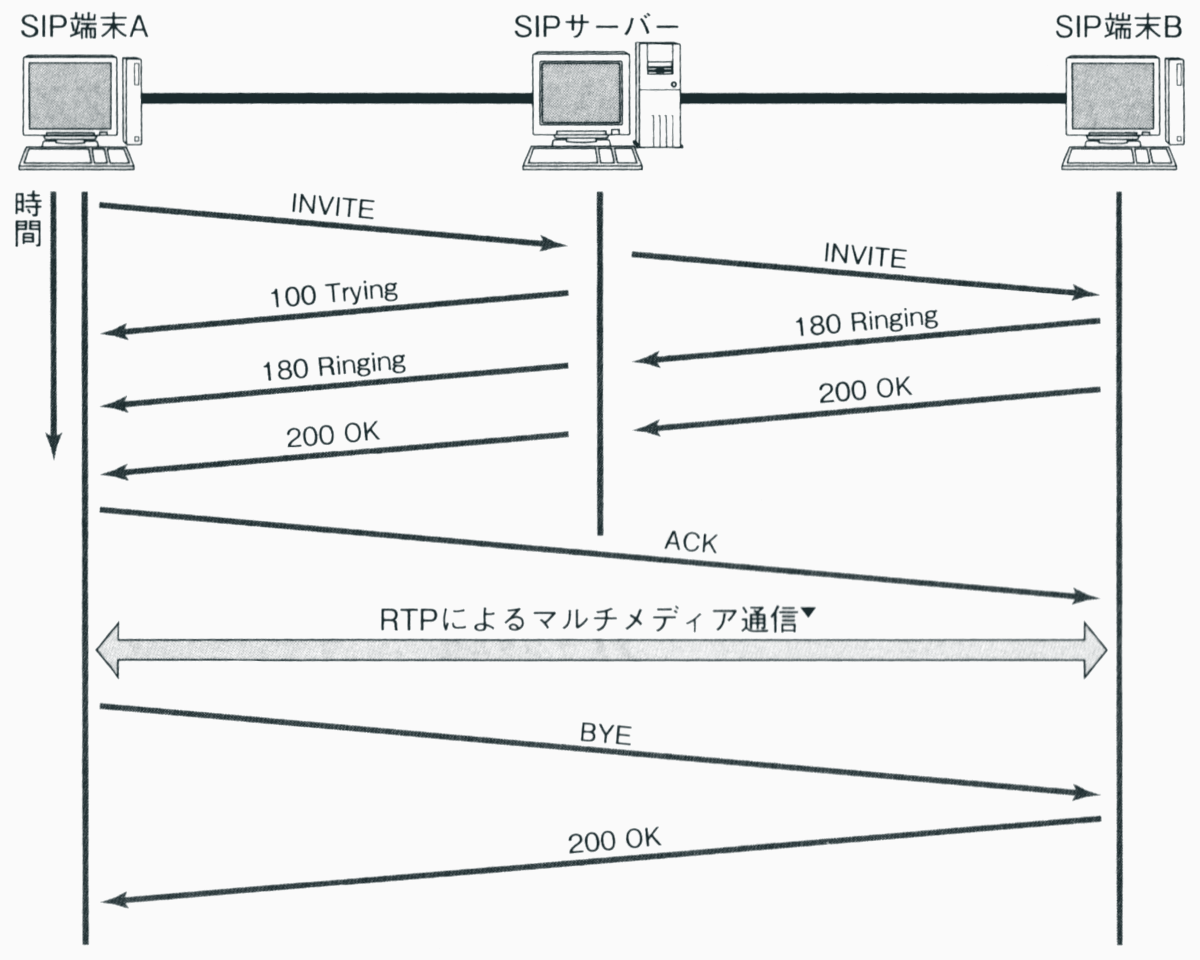
\includegraphics[height=.9\textheight]{./images/sip.png}
    \end{column}
  \end{columns}

  ~\\[-.9\baselineskip]
  {\tiny\raggedright
  井上直也,村山公保,竹下隆史,荒井 透,苅田幸雄:\\[-1.5\baselineskip]
  \raggedright
  第8章 アプリケーションプロトコル,
  「マスタリングTCP/IP 入門編(第6版)」,
  p.331,
  株式会社オーム社,2021.}
  \\~\\[3\baselineskip]

  \note{ }
\end{frame}

\begin{frame}
  \frametitle{どうしてSIPは届いてRTPは届かないのか}

  Firewallか何かが悪さをしていそう\\
  \hspace{1.5\zw}この局はTailscale ACLやMikoPBX Firewallをいじっていた\\
  \hspace{1.5\zw}Tailscale ACLはyude-MikaNeTEL間のことで嫌になっている
  \\~\\[-.5\baselineskip]

  いったん全ての武装を解除してみる\\
  \hspace{1.5\zw}Tailscale ACLをall allowに\\
  \hspace{1.5\zw}MikoPBX Firewallをdisabledに\\
  \hspace{1.5\zw}しかし改善せず(は?)→ 泥沼のスタート

  \note{ }
\end{frame}

\begin{frame}
  \frametitle{調べてみると片方向通信になる話が出てくる}

  NAPT環境下だと片方向通信になりがち\\
  \hspace{1.5\zw}NAPT環境で外から内に入ってくるには\\
  \hspace{1.5\zw}能動的に内から外に出る必要がある
  \\~\\[-.5\baselineskip]

  SIPの通信はこれに該当する\\
  \hspace{1.5\zw}SIPサーバはリクエストがあって初めて答えてくれる
  \\~\\[-.5\baselineskip]

  RTPの通信はこれに該当しない\\
  \hspace{1.5\zw}SIP上で指定されたポートを狙って勝手に飛んでくる\\
  \hspace{1.5\zw}NAPTは飛んできたパケットを誰に転送するのかわからない

  \note{ }
\end{frame}

\begin{frame}
  \frametitle{や、でもこれTailnet内の通信だよ?}

  あ、そうだったわ

  \note{ }
\end{frame}

\begin{frame}
  \frametitle{その他の関係ない人たち}

  上流がRakuten Turbo 5Gルータだよ?\\
  \hspace{1.5\zw}→ 同様の環境で疎通してる別の局がありました
  \\~\\[-.5\baselineskip]

  無線だからかRTTめちゃくちゃデカいよ?\\
  \hspace{1.5\zw}→ バカ遅いリンクでも他局と通信できました(10Base2)
  \\~\\[-.5\baselineskip]

  音声コーデック非対応なんじゃない?\\
  \hspace{1.5\zw}→ よく使われるものに絞ってもダメでした

  \note{ }
\end{frame}

\section{ええい、総当たりじゃ!}
\note{ }

\begin{frame}
  \frametitle{とりあえず全局と接続テストしてみる}

  東京広域電話網の全ての局で片方向通信になるのか確かめてみる\\
  \hspace{1.5\zw}通信できる局は比較的多かった\\
  \hspace{1.5\zw}むしろ片方向通信や不通になる方がレア
  \\~\\[-.5\baselineskip]

  通信できる他の局をホップしてから通信すると繋がる\\
  \hspace{1.5\zw}これに頼っても良いけどちょっと不便かも\\
  \hspace{1.5\zw}(スケールできないことを露呈していてダメ)
  \\~\\[-.5\baselineskip]

  とはいえ、原因となるものが何もわからない

  \note{ }
\end{frame}

\begin{frame}
  \frametitle{伝家の宝刀 パケットキャプチャ}

  \texttt{tcpdump}を使ってパケットを眺めてみる\\
  \hspace{1.5\zw}SIPのパケットは問題なさそうに見える\\
  \hspace{1.5\zw}予想通りRTPのパケットは片方しか来ていない
  \\~\\[-.5\baselineskip]

  しかもなんか変なNICに出てる\\
  \hspace{1.5\zw}Tailnet上の通信は仮想NIC(\texttt{tailscale0})に流れるハズ\\
  \hspace{1.5\zw}発狂している通信では物理NIC(\texttt{eth0})に流れている

  \note{ }
\end{frame}

\begin{frame}
  \frametitle{あぁ、ちゃんと100.70.198.29にパケット投げてるのに!}

  「え、100.70.198.29って誰ですか」
  \\~\\[2\baselineskip]

  「は?」

  \note{ }
\end{frame}

\begin{frame}
  \centering
  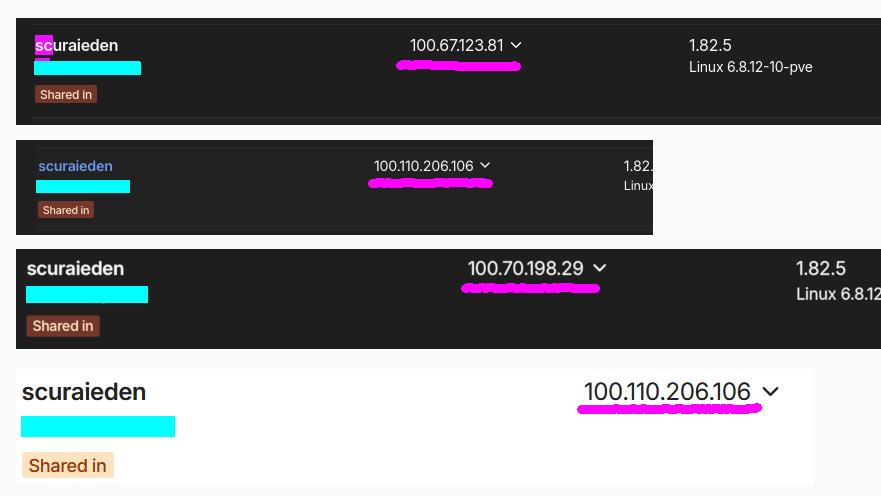
\includegraphics[height=.9\textheight]{./images/hakkyo.png}
\end{frame}

\begin{frame}
  \frametitle{TailscaleでIPv4アドレスを割り当て直すと通信可能に!}

  Tailscaleの機能でIPv4アドレスを再設定\\
  \hspace{1.5\zw}通信の両端で同じアドレスとなるように設定\\
  \hspace{1.5\zw}無事に通信できるようになりました
  \\~\\[-.5\baselineskip]

  \hfill ……本当か?

  \note{ }
\end{frame}

\section{考察・追実験}
\note{ }

\begin{frame}
  \frametitle{互いに異なるIPv4アドレスが見えていたため発狂した?}

  お互いに見えているIPv4アドレスが異なる事象\\
  \hspace{1.5\zw}Tailscaleがよしなにしているなら問題ないハズ\\
  \hspace{1.5\zw}つまり、TailscaleがNATのように仕事をしている?

  SIPで通信できたのはNAT的ふるまいのおかげ

  RTPはSIPで指定されたIPアドレス・ポートを使う\\
  \hspace{1.5\zw}指定された場所はルーティングテーブルに存在しない\\
  \hspace{1.5\zw}デフォルトルートである\texttt{eth0}にパケットをぶん投げる

  \note{ }
\end{frame}

\begin{frame}
  \frametitle{じゃあ追実験だ!}

  通信できている局間でIPv4アドレスを変えたら発狂するのか

  \begin{itemize}
    \item[1.]
      通信できている局の対を用意する
    \item[2.]
      片方のIPv4アドレスを変更してみる(発狂させる)
    \item[3.]
      通信が壊れる
    \item[4.]
      IPv4アドレスを直したら通信できるようになる
  \end{itemize}

  \note{ }
\end{frame}

\begin{frame}
  \frametitle{実験は失敗しました}

  \begin{itemize}
    \item[1.]
      通信できている局の対を用意する
    \item[2.]
      片方のIPv4アドレスを変更してみる(発狂させる)
    \item[3.]
      \dsout{通信が壊れる} ← \textbf{壊れませんでした}
    \item[4.]
      IPv4アドレスを直したら通信できるようになる
  \end{itemize}

  そもそも異なるIPv4アドレスが見えていたのに\\
  \hspace{1.5\zw}通信できていた局も存在していたのでした

  つまりルーティングテーブルにないホストと通信できている\\
  \hspace{1.5\zw}(もう何もわからん)

  \note{ }
\end{frame}

\section{まとめ}
\note{ }

\begin{frame}
  \frametitle{オレオレIP電話網を破壊したり発狂したりしてみた}

  分散形の異常オレオレIP電話網「東京広域電話網」

  ベルは鳴るのに音声が届かない問題を掘り下げた

  SIPとRTPとの通信の違いを確認した

  Tailscaleのせいなのか何なのかよくわからない感じになった

  ~\\[-.5\baselineskip]

  バックボーンの通信も自分で実現すれば発狂せずに済むかもネ\\
  \hspace{1.5\zw}東京広域通信網に乞うご期待
\end{frame}

\begin{frame}[standout]
  東京広域電話網は\\
  {\Huge 老練な\\ネットワークエンジニア}\\
  を募集しています\\[1\baselineskip]
  {\tiny 電話屋さん、懐古厨、カーネルエンジニア、信号処理屋さん、古代のコンピュータ技術者を含む一般人・逸般人も可}
  \\[-2\baselineskip]

  \note{ }
\end{frame}

\begin{frame}[standout]
  おわりです\\[3\baselineskip]
  {\small\mdseries \textit{Telephone for Everyone, Connecting Heritages}}
  \\[-4\baselineskip]
  \note{
    発表おわり〜
  }
\end{frame}

\begin{frame}
  \frametitle{このスライドについて}

  Written in May 2025.
  Updated in June 2025.
  \\~\\[-.5\baselineskip]

  Permanent ID of this document: \texttt{c8edfb391dbbafd3}.
  \\~\\[-.5\baselineskip]

  Copyright © 2025 KusaReMKN, 東京広域電話網.
  \\~\\[-.5\baselineskip]

  特記無き場合、プログラムやソースコードは MIT License で、\\
  \hspace{1.5\zw}それ以外のコンテンツは CC-BY 4.0 で利用可能です。\\
  \hspace{1.5\zw}一部の画像には別のライセンスが適用されるかもしれません。
\end{frame}

\end{document}
% ex: se et ts=2 :
